%% uncomment to list all files in log
%\listfiles

\documentclass[12pt]{report}


\usepackage{fontspec}

%\setmainfont[Scale=MatchLowercase]{Lucida Bright}
%\setmonofont{FreeMono}
%\setmonofont{Source Code Pro}
\setmonofont[Scale=MatchLowercase]{Ubuntu Mono}

\usepackage[headings]{fullpage}

% national use characters 
%\usepackage{inputenc}

% ams mathematical symbols
\usepackage{amsmath,amssymb}

% added to support pandoc highlighting
\usepackage{microtype}

\usepackage{makeidx}

% add index and bibliographies to table of contents
\usepackage[nottoc]{tocbibind}

% postscript courier and times in place of cm fonts
%\usepackage{courier}
%\usepackage{times}

% extended coloring
\usepackage{color}
\usepackage[table,dvipsnames]{xcolor}
\usepackage{colortbl}

% advanced date formating
\usepackage{datetime}

%support pandoc code highlighting
\usepackage{fancyvrb}
\DefineShortVerb[commandchars=\\\{\}]{\|}
\DefineVerbatimEnvironment{Highlighting}{Verbatim}{commandchars=\\\{\}}
% Add ',fontsize=\small' for more characters per line

%tango style colors
% \usepackage{framed}
% \definecolor{shadecolor}{RGB}{255,255,255}
% \newenvironment{Shaded}{\begin{snugshade}}{\end{snugshade}}
% \newcommand{\KeywordTok}[1]{\textcolor[rgb]{0.13,0.29,0.53}{\textbf{{#1}}}}
% \newcommand{\DataTypeTok}[1]{\textcolor[rgb]{0.13,0.29,0.53}{{#1}}}
% \newcommand{\DecValTok}[1]{\textcolor[rgb]{0.00,0.00,0.81}{{#1}}}
% \newcommand{\BaseNTok}[1]{\textcolor[rgb]{0.00,0.00,0.81}{{#1}}}
% \newcommand{\FloatTok}[1]{\textcolor[rgb]{0.00,0.00,0.81}{{#1}}}
% \newcommand{\CharTok}[1]{\textcolor[rgb]{0.31,0.60,0.02}{{#1}}}
% \newcommand{\StringTok}[1]{\textcolor[rgb]{0.31,0.60,0.02}{{#1}}}
% \newcommand{\CommentTok}[1]{\textcolor[rgb]{0.56,0.35,0.01}{\textit{{#1}}}}
% \newcommand{\OtherTok}[1]{\textcolor[rgb]{0.56,0.35,0.01}{{#1}}}
% \newcommand{\AlertTok}[1]{\textcolor[rgb]{0.94,0.16,0.16}{{#1}}}
% \newcommand{\FunctionTok}[1]{\textcolor[rgb]{0.00,0.00,0.00}{{#1}}}
% \newcommand{\RegionMarkerTok}[1]{{#1}}
% \newcommand{\ErrorTok}[1]{\textbf{{#1}}}
% \newcommand{\NormalTok}[1]{{#1}}

%espresso style colors
% \usepackage{framed}
% \definecolor{shadecolor}{RGB}{42,33,28}
% \newenvironment{Shaded}{\begin{snugshade}}{\end{snugshade}}
% \newcommand{\KeywordTok}[1]{\textcolor[rgb]{0.26,0.66,0.93}{\textbf{{#1}}}}
% \newcommand{\DataTypeTok}[1]{\textcolor[rgb]{0.74,0.68,0.62}{\underline{{#1}}}}
% \newcommand{\DecValTok}[1]{\textcolor[rgb]{0.27,0.67,0.26}{{#1}}}
% \newcommand{\BaseNTok}[1]{\textcolor[rgb]{0.27,0.67,0.26}{{#1}}}
% \newcommand{\FloatTok}[1]{\textcolor[rgb]{0.27,0.67,0.26}{{#1}}}
% \newcommand{\CharTok}[1]{\textcolor[rgb]{0.02,0.61,0.04}{{#1}}}
% \newcommand{\StringTok}[1]{\textcolor[rgb]{0.02,0.61,0.04}{{#1}}}
% \newcommand{\CommentTok}[1]{\textcolor[rgb]{0.00,0.40,1.00}{\textit{{#1}}}}
% \newcommand{\OtherTok}[1]{\textcolor[rgb]{0.74,0.68,0.62}{{#1}}}
% \newcommand{\AlertTok}[1]{\textcolor[rgb]{1.00,1.00,0.00}{{#1}}}
% \newcommand{\FunctionTok}[1]{\textcolor[rgb]{1.00,0.58,0.35}{\textbf{{#1}}}}
% \newcommand{\RegionMarkerTok}[1]{\textcolor[rgb]{0.74,0.68,0.62}{{#1}}}
% \newcommand{\ErrorTok}[1]{\textcolor[rgb]{0.74,0.68,0.62}{\textbf{{#1}}}}
% \newcommand{\NormalTok}[1]{\textcolor[rgb]{0.74,0.68,0.62}{{#1}}}

%kete style colors
% \newenvironment{Shaded}{}{}
% \newcommand{\KeywordTok}[1]{\textbf{{#1}}}
% \newcommand{\DataTypeTok}[1]{\textcolor[rgb]{0.50,0.00,0.00}{{#1}}}
% \newcommand{\DecValTok}[1]{\textcolor[rgb]{0.00,0.00,1.00}{{#1}}}
% \newcommand{\BaseNTok}[1]{\textcolor[rgb]{0.00,0.00,1.00}{{#1}}}
% \newcommand{\FloatTok}[1]{\textcolor[rgb]{0.50,0.00,0.50}{{#1}}}
% \newcommand{\CharTok}[1]{\textcolor[rgb]{1.00,0.00,1.00}{{#1}}}
% \newcommand{\StringTok}[1]{\textcolor[rgb]{0.87,0.00,0.00}{{#1}}}
% \newcommand{\CommentTok}[1]{\textcolor[rgb]{0.50,0.50,0.50}{\textit{{#1}}}}
% \newcommand{\OtherTok}[1]{{#1}}
% \newcommand{\AlertTok}[1]{\textcolor[rgb]{0.00,1.00,0.00}{\textbf{{#1}}}}
% \newcommand{\FunctionTok}[1]{\textcolor[rgb]{0.00,0.00,0.50}{{#1}}}
% \newcommand{\RegionMarkerTok}[1]{{#1}}
% \newcommand{\ErrorTok}[1]{\textcolor[rgb]{1.00,0.00,0.00}{\textbf{{#1}}}}
% \newcommand{\NormalTok}[1]{{#1}}
%end pandoc code hacks

% jodliterate colors
\usepackage{color}
\definecolor{shadecolor}{RGB}{248,248,248}
% j control structures 
\definecolor{keywcolor}{rgb}{0.13,0.29,0.53}
% j explicit arguments x y m n u v
\definecolor{datacolor}{rgb}{0.13,0.29,0.53}
% j numbers - all types see j.xml
\definecolor{decvcolor}{rgb}{0.00,0.00,0.81}
\definecolor{basencolor}{rgb}{0.00,0.00,0.81}
\definecolor{floatcolor}{rgb}{0.00,0.00,0.81}
% j local assignments
\definecolor{charcolor}{rgb}{0.31,0.60,0.02}
\definecolor{stringcolor}{rgb}{0.31,0.60,0.02}
\definecolor{commentcolor}{rgb}{0.56,0.35,0.01}
% primitive adverbs and conjunctions
%\definecolor{othercolor}{rgb}{0.56,0.35,0.01}   
\definecolor{othercolor}{RGB}{0,0,255}
% global assignments
\definecolor{alertcolor}{rgb}{0.94,0.16,0.16}
% primitive J verbs and noun names
\definecolor{funccolor}{rgb}{0.00,0.00,0.00}    

\usepackage{framed}
\newenvironment{Shaded}{}{}
\newcommand{\KeywordTok}[1]{\textcolor{keywcolor}{\textbf{{#1}}}}
\newcommand{\DataTypeTok}[1]{\textcolor{datacolor}{{#1}}}
%\newcommand{\DecValTok}[1]{\textcolor{decvcolor}{{#1}}}
\newcommand{\DecValTok}[1]{{#1}} 
\newcommand{\BaseNTok}[1]{\textcolor{basencolor}{{#1}}}
\newcommand{\FloatTok}[1]{\textcolor{floatcolor}{{#1}}}
\newcommand{\CharTok}[1]{\textcolor{charcolor}{\textbf{{#1}}}}
\newcommand{\StringTok}[1]{\textcolor{stringcolor}{{#1}}}
\newcommand{\CommentTok}[1]{\textcolor{commentcolor}{\textit{{#1}}}}
\newcommand{\OtherTok}[1]{\textcolor{othercolor}{{#1}}} 
\newcommand{\AlertTok}[1]{\textcolor{alertcolor}{\textbf{{#1}}}}
%\newcommand{\FunctionTok}[1]{\textcolor{funccolor}{{#1}}}
\newcommand{\FunctionTok}[1]{{#1}}
\newcommand{\RegionMarkerTok}[1]{{#1}}
\newcommand{\ErrorTok}[1]{\textbf{{#1}}}
\newcommand{\NormalTok}[1]{{#1}}

% headers and footers
\usepackage{fancyhdr}
\pagestyle{fancy}

\fancyhead{}
\fancyfoot{}

%\fancyhead[LE,RO]{\slshape \rightmark}
%\fancyhead[LO,RE]{\slshape \leftmark}
\fancyfoot[C]{\thepage}
%\headrulewidth 0.4pt
%\footrulewidth 0 pt

%\addtolength{\headheight}{\baselineskip}

%\lfoot{\emph{Analyze the Data not the Drivel}}
%\rfoot{\emph{\today}}

% subfigure handles figures that contain subfigures
%\usepackage{color,graphicx,subfigure,sidecap}
\usepackage{graphicx,sidecap}
\usepackage{subfigure}
\graphicspath{{./inclusions/}}

% floatflt provides for text wrapping around small figures and tables
\usepackage{floatflt}

% tweak caption formats 
\usepackage{caption} 
\usepackage{sidecap}
%\usepackage{subcaption} % not compatible with subfigure

\usepackage{rotating} % flip tables sideways

% complex footnotes
%\usepackage{bigfoot}

% weird logos \XeLaTeX
\usepackage{metalogo}

% source code listings
\usepackage{listings}

% long tables
% \usepackage{longtable}

\newcommand{\HRule}{\rule{\linewidth}{0.5mm}}

% map LaTeX cross references into PDF cross references
\usepackage[
            %dvips,
            colorlinks,
            linkcolor=blue,
            citecolor=blue,
            urlcolor=blue,   % magenta, cyan default        
            pdfauthor={John D. Baker},
            pdftitle={Analyze the Data not the Drivel},
            pdfsubject={Blog},
            pdfcreator={MikTeX+LaTeXe with hyperref package},
            pdfkeywords={blog,wordpress},
            ]{hyperref}
           
% custom colors
\definecolor{CodeBackGround}{cmyk}{0.0,0.0,0,0.05}    % light gray
\definecolor{CodeComment}{rgb}{0,0.50,0.00}           % dark green {0,0.45,0.08}
\definecolor{TableStripes}{gray}{0.9}                 % odd/even background in tables

\lstdefinelanguage{bat}
{morekeywords={echo,title,pushd,popd,setlocal,endlocal,off,if,not,exist,set,goto,pause},
sensitive=True,
morecomment=[l]{rem}
}

\lstdefinelanguage{jdoc}
{
morekeywords={},
otherkeywords={assert.,break.,continue.,for.,do.,if.,else.,elseif.,return.,select.,end.
,while.,whilst.,throw.,catch.,catchd.,catcht.,try.,case.,fcase.},
sensitive=True,
morecomment=[l]{NB.},
morestring=[b]',
morestring=[d]',
}

% latex size ordering - can never remember it
% \tiny
% \scriptsize
% \footnotesize
% \small
% \normalsize
% \large
% \Large
% \LARGE
% \huge
% \Huge
 
% listings package settings  
\lstset{%
  language=jdoc,                                % j document settings
  basicstyle=\ttfamily\footnotesize,            
  keywordstyle=\bfseries\color{keywcolor}\footnotesize,
  identifierstyle=\color{black},
  commentstyle=\slshape\color{CodeComment},     % colored slanted comments
  stringstyle=\color{red}\ttfamily,
  showstringspaces=false,                       
  %backgroundcolor=\color{CodeBackGround},       
  frame=single,                                
  framesep=1pt,                                 
  framerule=0.8pt,                             
  rulecolor=\color{CodeBackGround},   
  showspaces=false,
  %columns=fullflexible,
  %numbers=left,
  %numberstyle=\footnotesize,
  %numbersep=9pt,
  tabsize=2,
  showtabs=false,
  captionpos=b
  breaklines=true,                              
  breakindent=5pt                              
}

\lstdefinelanguage{JavaScript}{
  keywords={typeof, new, true, false, catch, function, return, null, catch, switch, var, if, in, while, do, else, case, break},
  ndkeywords={class, export, boolean, throw, implements, import, this},
  ndkeywordstyle=\color{darkgray}\bfseries,
  sensitive=false,
  comment=[l]{//},
  morecomment=[s]{/*}{*/},
  morestring=[b]',
  morestring=[b]"
}

% C# settings
\lstdefinestyle{sharpc}{
language=[Sharp]C,
basicstyle=\ttfamily\scriptsize, 
keywordstyle=\bfseries\color{keywcolor}\scriptsize,
framerule=0pt
}

% for source code listing longer than two use smaller font
\lstdefinestyle{smallersource}{
basicstyle=\ttfamily\scriptsize, 
keywordstyle=\bfseries\color{keywcolor}\scriptsize,
framerule=0pt
}

\lstdefinestyle{resetdefaults}{
language=jdoc,
basicstyle=\ttfamily\footnotesize,  
keywordstyle=\bfseries\color{keywcolor}\footnotesize,                                                               
framerule=0.8pt 
}

% APL UTF8 code points listed for lstlisting processing
\makeatletter
\lst@InputCatcodes
\def\lst@DefEC{%
 \lst@CCECUse \lst@ProcessLetter
  ^^80^^81^^82^^83^^84^^85^^86^^87^^88^^89^^8a^^8b^^8c^^8d^^8e^^8f%
  ^^90^^91^^92^^93^^94^^95^^96^^97^^98^^99^^9a^^9b^^9c^^9d^^9e^^9f%
  ^^a0^^a1^^a2^^a3^^a4^^a5^^a6^^a7^^a8^^a9^^aa^^ab^^ac^^ad^^ae^^af%
  ^^b0^^b1^^b2^^b3^^b4^^b5^^b6^^b7^^b8^^b9^^ba^^bb^^bc^^bd^^be^^bf%
  ^^c0^^c1^^c2^^c3^^c4^^c5^^c6^^c7^^c8^^c9^^ca^^cb^^cc^^cd^^ce^^cf%
  ^^d0^^d1^^d2^^d3^^d4^^d5^^d6^^d7^^d8^^d9^^da^^db^^dc^^dd^^de^^df%
  ^^e0^^e1^^e2^^e3^^e4^^e5^^e6^^e7^^e8^^e9^^ea^^eb^^ec^^ed^^ee^^ef%
  ^^f0^^f1^^f2^^f3^^f4^^f5^^f6^^f7^^f8^^f9^^fa^^fb^^fc^^fd^^fe^^ff%
  ^^^^20ac^^^^0153^^^^0152%
  ^^^^20a7^^^^2190^^^^2191^^^^2192^^^^2193^^^^2206^^^^2207^^^^220a%
  ^^^^2218^^^^2228^^^^2229^^^^222a^^^^2235^^^^223c^^^^2260^^^^2261%
  ^^^^2262^^^^2264^^^^2265^^^^2282^^^^2283^^^^2296^^^^22a2^^^^22a3%
  ^^^^22a4^^^^22a5^^^^22c4^^^^2308^^^^230a^^^^2336^^^^2337^^^^2339%
  ^^^^233b^^^^233d^^^^233f^^^^2340^^^^2342^^^^2347^^^^2348^^^^2349%
  ^^^^234b^^^^234e^^^^2350^^^^2352^^^^2355^^^^2357^^^^2359^^^^235d%
  ^^^^235e^^^^235f^^^^2361^^^^2362^^^^2363^^^^2364^^^^2365^^^^2368%
  ^^^^236a^^^^236b^^^^236c^^^^2371^^^^2372^^^^2373^^^^2374^^^^2375%
  ^^^^2377^^^^2378^^^^237a^^^^2395^^^^25af^^^^25ca^^^^25cb%  
  ^^00}
\lst@RestoreCatcodes
\makeatother

% custom lengths used within minipages
\newcommand{\minindent}{17pt}


\makeindex

\begin{document}

\subsection*{\href{http://analyzethedatanotthedrivel.org/2017/01/22/affinity-photo-review/}{Affinity Photo Review}}
\addcontentsline{toc}{subsection}{Affinity Photo Review}


\noindent\emph{Posted: 22 Jan 2017 23:40:20}
\vspace{6pt}

There's a new image processor on my computers. Recently the chief
developer of one of my favorite image editors,
\href{http://www.dl-c.com/}{Picture Window Pro} (PWP), sent out a sad
email letting all PWP users know that he is stopping PWP development. He
thanked us for over twenty years of support and as a last gift converted
the final version of PWP to freeware. You can now download and run
Picture Window Pro without a key. PWP is a superb program! It's still
the fastest and meanest image editor I have ever used and I am
constantly trying image editors. If you're interested in getting a free
copy of PWP download the program before the distribution website shuts
down.

I was saddened by this news but all good things eventually end. With PWP
going away I decided, for the n\textsuperscript{th} time, to look for
alternatives. I reconsidered Photoshop. I've used full-blown Photoshop
but frankly, I've never been impressed. It's expensive and slow! I use
an old copy of Photoshop Elements, mainly to remove blemishes on film
scans, but in my opinion, the only Adobe image processing product worth
paying for is
\href{https://www.adobe.com/products/photoshop-lightroom.html}{Lightroom}.
Adobe is the evil image processing empire. They squeeze you with
sluggish performance and abusive subscription payment models and then
act like they're doing you a favor. It didn't take me very long to
abandon Photoshop (again) and keep looking for PWP alternatives. Lucky
for me there's this thing called
\href{https://start.duckduckgo.com/}{DuckDuckGo} that quickly led me to
\href{https://affinity.serif.com/en-us/}{Affinity Photo.}

Affinity Photo is a relatively new image editor that got started in the
Mac world and, as of November 2016, is also available for 64 bit Windows
systems. Affinity has snagged dozens of
\href{https://fstoppers.com/photoshop/affinity-photo-finally-true-alternative-photoshop-windows-153211}{positive
reviews} and, unlike Photoshop, is reasonably priced. I decided to give
myself a little Christmas present and bought Affinity Photo.

The Affinity Windows download file is large: over 200 megabytes.
Affinity Windows depends on \texttt{.Net\ 4.6.2} which is also
installed if it's not on your machine. It took a few minutes to suck
down and install all the required bytes but things went smoothly and I
eagerly started the program.

Before relating my impressions of Affinity Photo I will describe my
\emph{binary image format philosophy}. Image editors typically create
and manipulate vendor specific proprietary binary image files. Binary
image files like PSDs, NEFs, DNGs, and now Affinity's AFPHOTOs, have a
nasty tendency to evolve on vendor whim. This poses fundamental
long-term image storage problems. Even if you conscientiously backup and
archive your original image files you may discover, a decade hence, that
you can no longer load them with current software. I hate this!
\emph{Photography is for the ages, not the marketing cycles of software
and camera companies!} If you have ever wondered why the lowly JPG image
format still reigns supreme despite its abundant technical deficiencies
stop wondering. The JPG format is an open and well described eight-bit
channel format. Any competent programmer can write software to read and
write JPGs. The same holds for TIFs, PNGs and a few other open formats.
This is not true for vendor dominated formats. The specifications, even
if disclosed, can change on a moment's notice.

How can photographers deal with \emph{transient} binary image formats?
There are two basic approaches. You can convert all your images to an
open image format. Some photographers convert camera RAW files to high
bit TIFs. Converting large numbers of image files is a tedious and
resource hungry process but it's probably the best bet for long-term
storage. I use the second lazier approach: maintain at least two
independent image programs that can read and write the binary image
formats you work with. I use Nikon cameras; they crank out proprietary
NEF binaries. Currently, I have four programs on this machine that can
read NEFs: PWP, Lightroom, Affinity and
\href{http://www.cerious.com/}{ThumbsPlus}. I will tolerate proprietary
binaries \emph{if and only if} I have options. Don't let software and
camera companies box you in.

I started using image editors about fifteen years ago. My first editor
came with my first digital camera: a one megapixel HP. I cannot remember
the name of this program; I only used it long enough to discover its
appalling deficiencies. Within a week I had purchased my first version
of Photoshop Elements (PE). I was happy with PE until I encountered
\href{https://en.wikipedia.org/wiki/Posterization}{posterization} (read
the link for the gory technical details). Posterization wreaks prints
and it's easy to posterize eight-bit channel images. The answer then, as
it is now, is to increase your working bit depth. Adobe recommended
upgrading from PE to full Photoshop. Why fork over \$70 bucks when you
can fork over \$500? Photoshop Elements has a long history of half-assed
support for sixteen-bit channel images and the reason is painfully
obvious. If Photoshop Elements fully embraced sixteen-bit channel images
there would be very little need for full Photoshop. You could save
yourself hundreds of dollars. Adobe decided not to compete with
themselves and adopted the time-tested pseudo-monopolistic practice of
sodomizing the customer. I did not embrace the
\href{http://www.urbandictionary.com/define.php?term=ButtHurt}{butthurt}!
I started looking for low-cost programs that properly handled
sixteen-bit images. It didn't take me long to find PWP.

This early experience shaped my entire image processing approach.
Instead of adopting a single monolithic ``industry standard'' program
and joining the \emph{nerd herd} I decided to go my way and use many
small programs. Instead of a Goliath, I went with many %\protect\hyperlink{fn1}{\textsuperscript{1}}
Davids.\footnote{If you remember what happened to Goliath siding with David doesn't
seem like much of a risk.} When you take the
David approach interoperability moves to the top of the stack. The
output of one program must effortlessly become the input of another. How
programs play together matters. Additionally, when you apply the David
approach, you never look to completely replace your tool set. General
purpose tools like Affinity may be able to do all the things more
specialized tools can do but probably not as efficiently or as well.

So, before adding Affinity to my trusted tools I asked:

\begin{enumerate}
\itemsep1pt\parskip0pt\parsep0pt
\def\labelenumi{\arabic{enumi}.}
%\tightlist
\item
  Does Affinity play nice with others?
\item
  Is Affinity's user interface (UI) tolerable?
\item
  Does Affinity streamline common tedious tasks?
\item
  What new capabilities does Affinity offer?
\end{enumerate}

With these points in mind let's look at Affinity Photo.

%\section*{Does Affinity play nice with others?}

\medskip
\noindent\textbf{Does Affinity play nice with others?}
\medskip

One of the first things I look for in image processors is
\emph{tolerable} loading times. Part the reason I've never been able to
stick with full Photoshop is because it takes forever to get the damn
thing up. Affinity on Windows easily beats full Photoshop but it's still
slower than good old C coded PWP. PWP comes up in a flash. It's one of
the many reasons I stuck with it for over a decade. Affinity's loading
speed is comparable to \href{https://www.gimp.org/}{GIMP}, Photoshop
Elements and Lightroom: fast enough to not drive me crazy.

After loading Affinity, I immediately started testing the program's
ability to read and write sixteen-bit TIF files. The basic single layer
sixteen-bit TIF file format is one of the best supported lossless image
formats. It's often the only way to move information from one program to
another without trashing bits. JPGs are universal, but every time you
write a JPG you lose data: that's the
\href{http://www.howtogeek.com/142174/what-lossless-file-formats-are-why-you-shouldnt-convert-lossy-to-lossless/}{lossy
part of JPG} compression. Lossy image formats are fine for the web and
final presentation but are a total disaster for image editing. Affinity
can read and write sixteen-bit TIFs. It can also read and write a number
of other important formats like Photoshop Elements PSDs. Affinity
converts PSD layers to AFPHOTO layers. It also handles JPGs, PNGs and
many RAW formats like Nikon's NEFs. \emph{Affinity plays well with
others.}

%\section*{Is Affinity's user interface UI tolerable?}

\medskip
\noindent\textbf{Is Affinity's user interface UI tolerable?}
\medskip


Once I had satisfied myself that I could slosh bits through Affinity I
started evaluating the program's user interface. UIs have ruined many
editors. I'm immediately suspicious when reviewers start lauding a
program's UI before spending a few hundred hours using it. UIs either
help or hinder. Affinity's UI is decent. If you have ever used a layer
oriented image editor you will quickly adjust to how Affinity works.
\href{https://affinity.serif.com/forum/index.php?/topic/10119-in-house-affinity-photo-video-tutorials/}{I
strongly recommend watching the Affinity tutorial videos}; they are
among the best video tutorials I've seen and quickly show what the
program can do.

Once Affinity is loaded it's pretty zippy. Common image handling
operations are fast enough to \emph{fly under my annoyance radar}. Image
processing can be very demanding. Don't expect to stitch 500-megabyte
panoramas from original RAW files instantly. With current hardware and
software, some things will take time. It's fair to say that Affinity's
performance compares favorably to other image processors. \emph{I can
put up with Affinity's user interface.}

%\section*{Does Affinity streamline common tedious tasks?}

\medskip
\noindent\textbf{Does Affinity streamline common tedious tasks?}
\medskip


After playing with Affinity for a few days I used the program to help
restore some old scanned slides. Old pictures are always damaged; they
all need a bit, or a lot, of retouching. The problems most people
associate with old pictures, tears, color changes, and loss of tone are
usually easily fixed in most editors. The biggest job is removing
thousands of scratches, spots, and stains. Most restorers give up and
crop or blur away such defects but I'm with Lady Macbeth: ``out, out
damn spots.'' Any tool that helps me hunt down and exterminate spotty
pests will be lovingly embraced.

The Affinity \href{https://vimeo.com/130966523}{inpainting brush} works
a lot better than the corresponding Photoshop Elements healing brush. In
particular, it crosses linear backgrounds, buildings, fabric patterns,
and so forth without unduly destroying detail. Removing long linear
scratches that cross regular structured detail is a soul draining chore.
Whenever I see such defects I typically give up and find another picture
to restore; I have a big backlog of scans awaiting restoration! This
slide (see page~\pageref{fig:5317X0}) of the southern end of Beirut Lebanon, taken by my


%{[}caption id=``attachment\_5316'' align=``aligncenter''  width=``584''{]}
\captionsetup[figure]{labelformat=empty}
\begin{figure}[htbp]
\centering
\href{https://conceptcontrol.smugmug.com/Places/Overseas-Places/Beirut-Lebanon-1960s-1/i-xVRksrK/A}{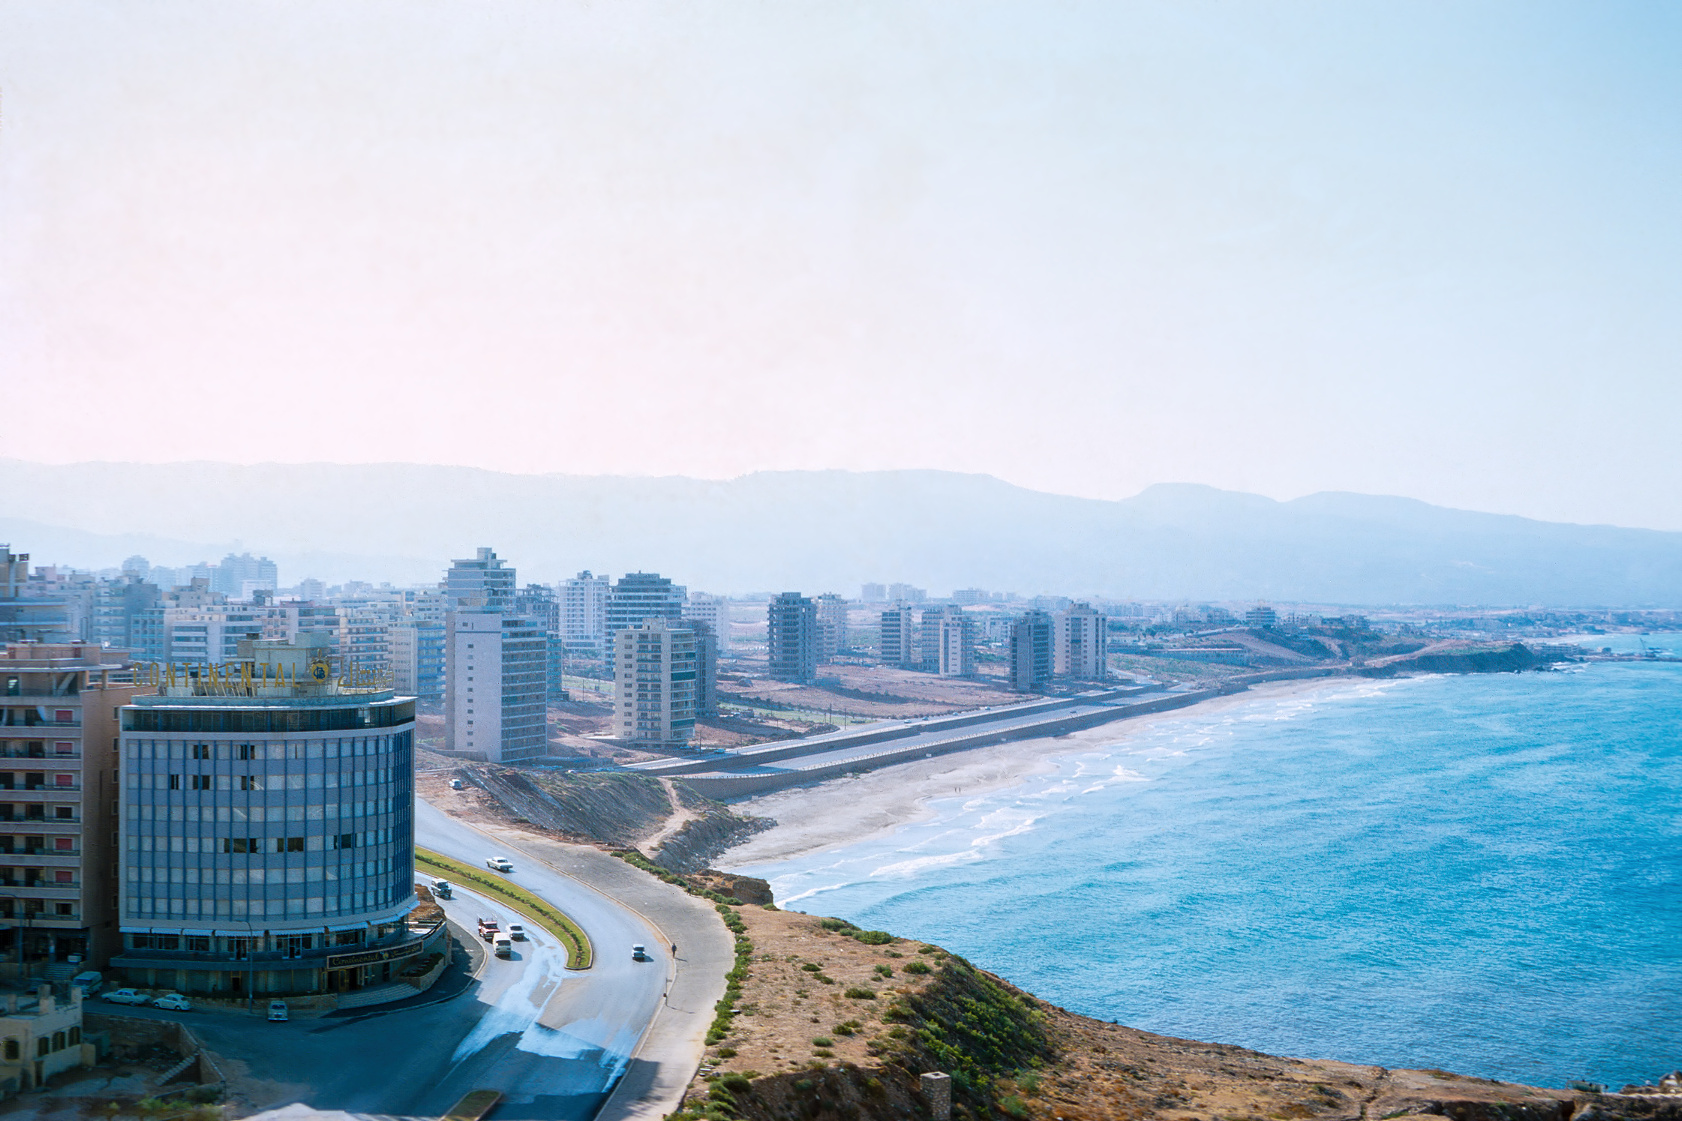
\includegraphics[width=6.08333in,height=4.05208in]{beirutsouthcoast.jpg}}
\caption{I am still exploring the Affinity Photo image editor. I used it to
restore this scan of a Kodachrome slide my father shot from a hotel
window of the south coast of Beirut Lebanon in 1968. The Continental
Hotel is visible in the lower left corner of this image. My mother often
stayed in the Continental when she visited me in Beirut. I fondly
remember having continental breakfast in the Continental. The original
slide was overexposed and covered with splotches and sky fingerprints.
The retouching tools in Affinity Photo are better than corresponding
tools in Photoshop Elements. I particularly like the Affinity inpainting
brush; it works well on textured and linear subjects. I was able to
remove long scratches cutting through the buildings in this image
without unduly wreaking building detail. I also used the inpainting tool
to remove a cutoff street light and a car it was shading on the bottom
of the image. It's easier to remove objects with Affinity Photo than it
is in Photoshop Elements.}
\label{fig:5317X0}
\end{figure}



father in 1968, is typical of many images in my backlog. There were
dozens of long linear scratches running through the buildings. It would
have taken hours to fix them with PE. All it took was a few passes with
Affinity's inpainting brush to remove them. I was impressed. This single
tool significantly speeds up restoring scratched and spotted images and
justifies Affinity's purchase price all by itself.

Another Affinity tool that streamlines common image processing tasks is
the Affinity panorama tool. Most modern image editors have fairly decent
panorama tools and building a panorama is easier than it used to be. In
the image editing Dark Age, you had to manually select control points
and master blend masks to build decent panoramas. It could take hours to
align a single image. Current editors use effective automatic control
point detection and advanced blending algorithms. In most cases, it's a
simple matter of using good capture technique followed by loading the
individual images into a panorama tool to generate decent to excellent
results.

We are living in a panoramic golden age but there are still problems. I
shoot entirely in RAW because RAW preserves the most information and
affords the greatest post processing options. Panoramas often encompass
scenes of high contrast. Image tones will vary from extremely bright to
very dark. It's not uncommon for ordinary panoramas to span twelve or
more stops of dynamic range. When processing high dynamic range pictures
it's extremely advantageous to do all your work on sixteen-bit or
thirty-two-bit channel images. Blending eight-bit panoramas
can~release\href{https://www.youtube.com/watch?v=7SqC_m3yUDU}{~\emph{the
posterization Kraken}}; trust me, you don't want that monster savaging
your scenes.

Unfortunately, the Photoshop Elements panorama tool is inherently
eight-bit. This means I must do all my major tone adjustments in
Lightroom before panorama stitching. Adjusting the tones of a single
image is tedious, doing it for many panorama frames is cruel and unusual
punishment. Adobe's answer is always the same; give us a lot of money
and we'll release you from eight-bit Hell! Lucky for us Affinity gets us
out of eight-bit panorama Hell for a lot less.

This panorama (see page~\pageref{fig:5317X1}) of the mountains near the eastern entrance of
Glacier National Park was directly generated from Nikon NEF RAW files.
All feature detection and blending calculations were high-bit. Tone
adjustments were aided by \href{https://vimeo.com/192632826}{regular
tone mapping}. Tone mapping is like an automatic
\href{https://en.wikipedia.org/wiki/Zone_System}{Zone System}. Compared
to what I used to put up with
\href{https://conceptcontrol.smugmug.com/Trips/USA-and-Canada/Arizona-Toodling-1/i-fMPPrqd/A}{ten
years ago} Affinity panorama building is almost as easy as scanning
scenes
\href{https://conceptcontrol.smugmug.com/Themes/Manipulations/Panoramas-1/i-phFMbnJ/A}{with
an iPhone}. \emph{Affinity significantly streamlines routine retouching
and panorama building.}


%{[}caption id=``attachment\_5315'' align=``aligncenter''  width=``584''{]}

\begin{figure}[htbp]
\centering
\href{https://conceptcontrol.smugmug.com/Themes/Manipulations/Panoramas-1/i-DDThBLs/A}{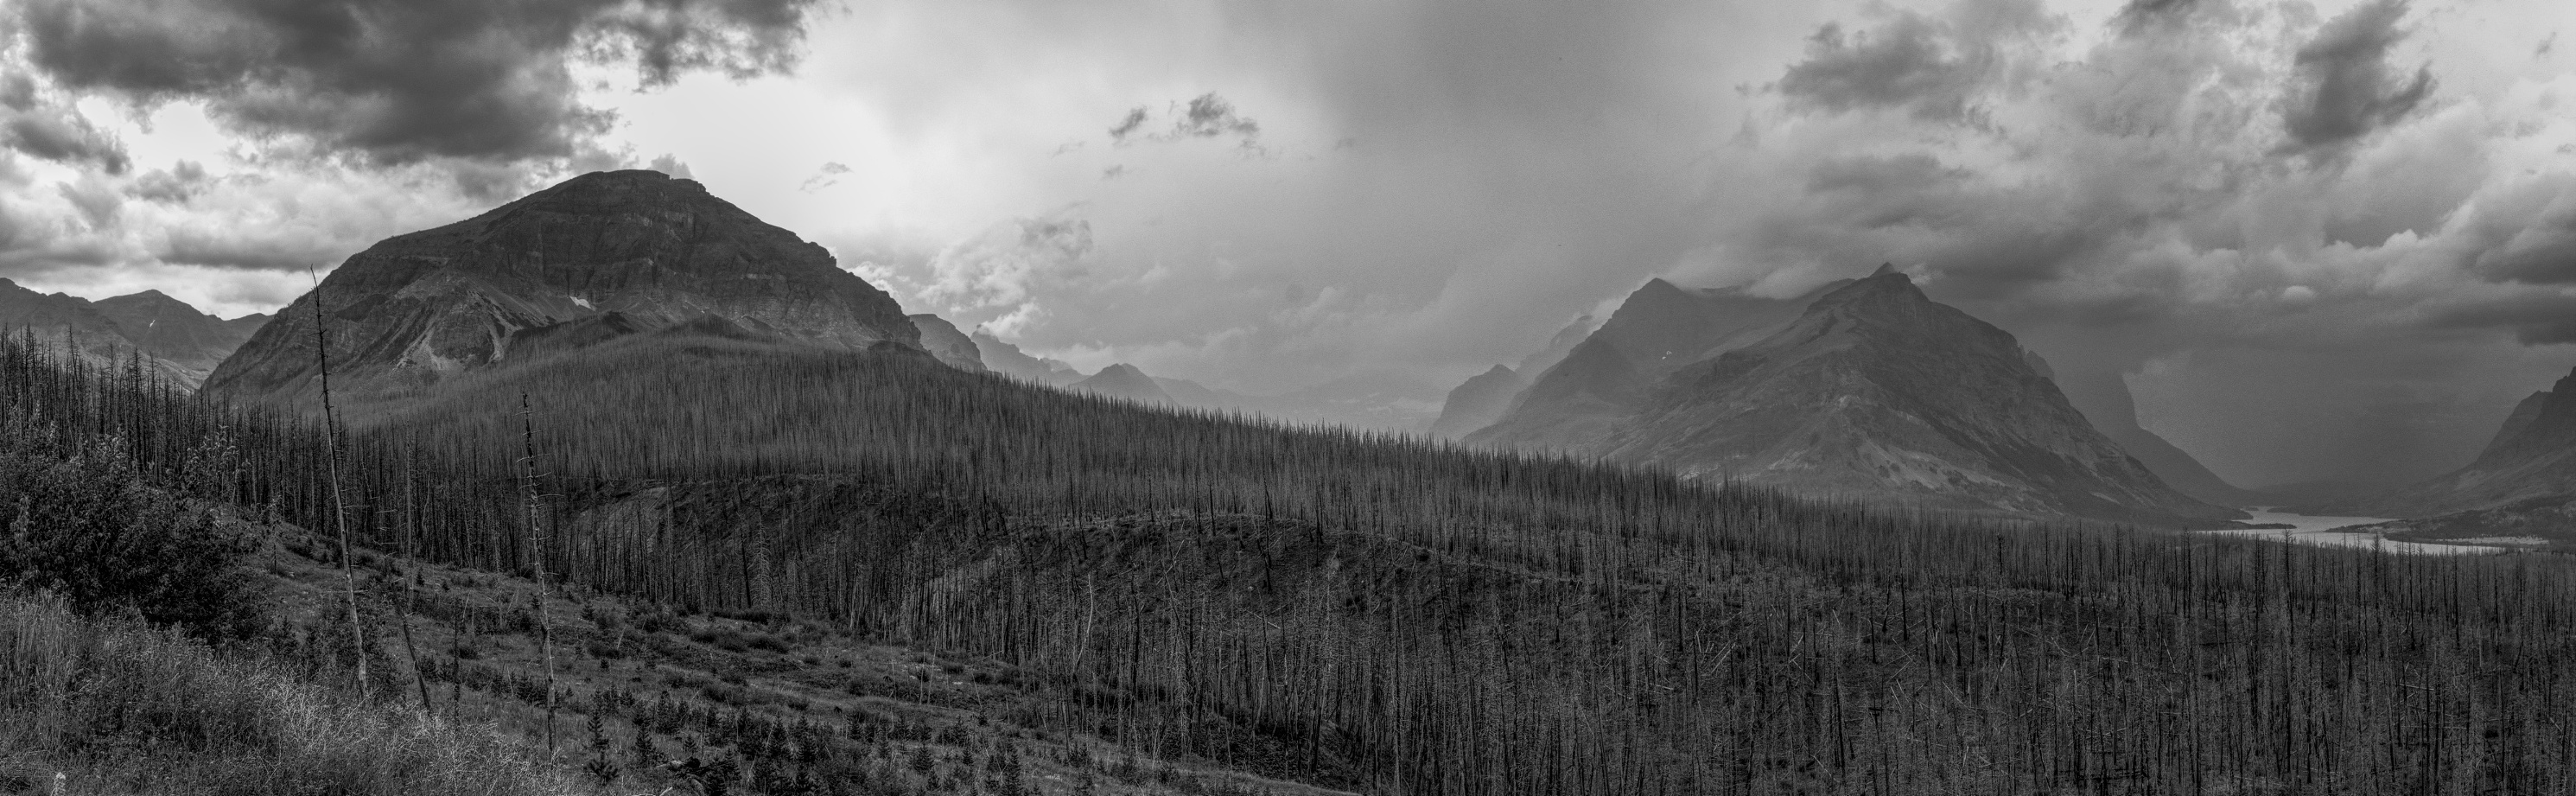
\includegraphics[width=6.08333in,height=1.87500in]{glaciermountainstorm.jpg}}
\caption{Looking west from just outside the eastern side of Glacier National Park
near Saint Mary. The weather was grim and dark, just the way I like it
when I braved the rain to snap the frames that went into this panorama.
I built this panorama directly from Nikon NEF files in the Windows
version of Affinity Photo. My favorite image processor, Picture Window
Pro, is being retired and I am exploring alternatives. I rather like
this result.}
\label{fig:5317X1}
\end{figure}


%\section*{What new capabilities does Affinity offer?}

\medskip
\noindent\textbf{What new capabilities does Affinity offer?}
\medskip

So far, the features I've discussed are common to most image editors.
Does Affinity offer anything new or special? There is one Affinity
feature, the~\emph{FFT (Fast Fourier Transform) Denoise filter}, that
greatly mitigates one of my long-standing retouching nightmares: regular
patterns.

Many old portraits were printed on patterned paper. This image (see page~\pageref{fig:5317X2}) is a
crop of an old (1935) baby picture of my mother.


%{[}caption id=``attachment\_5314'' align=``aligncenter''  width=``400''{]}

\begin{figure}[htbp]
\centering
\href{https://bakerjd99.files.wordpress.com/2017/01/evelynpattern.jpg}{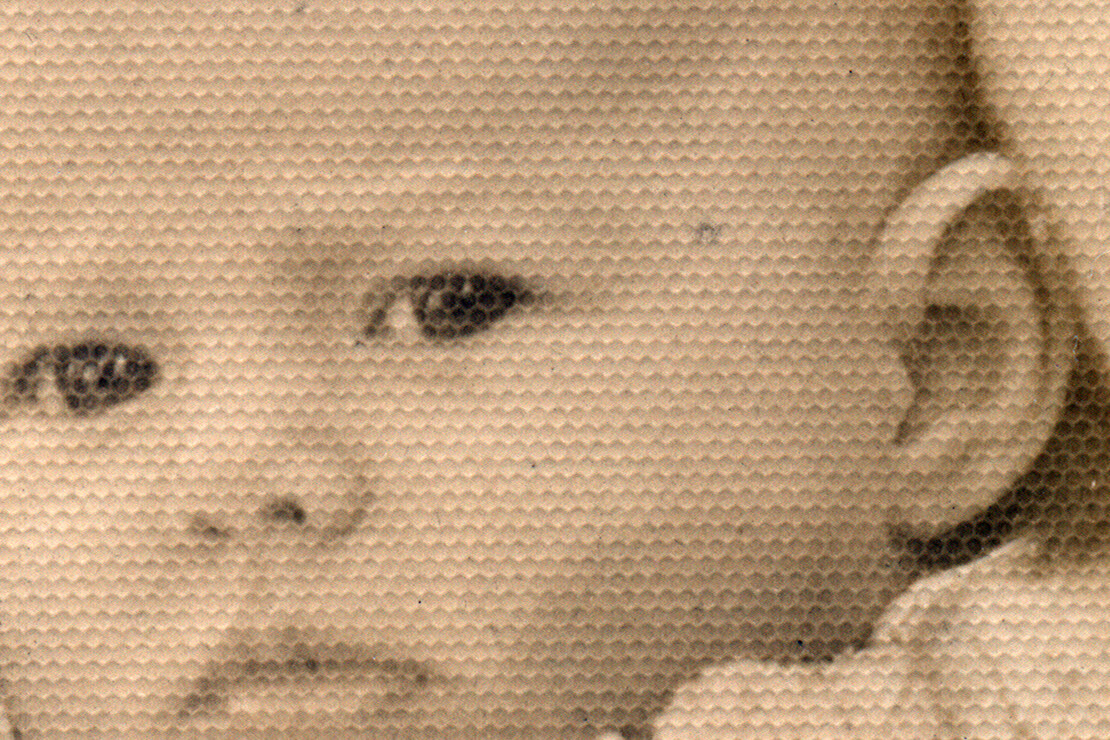
\includegraphics[width=4.16667in,height=2.78125in]{evelynpattern.jpg}}
\caption{My mother as a seven-week-old baby. This 1935 picture was printed on
patterned paper. Patterned paper often adds luster and depth to
photographs but it also makes it more difficult to retouch them. The
Affinity Photo FFT (Fast Fourier Transform) Denoise filter can remove
regular patterns without unduly softening images.}
\label{fig:5317X2}
\end{figure}



As you can see the entire picture is covered with tiny regular hexagons.
Patterned prints were popular in the early and
mid-20\textsuperscript{th} century. The pattern adds depth and luster
and has the nice side effect of making prints difficult to copy.
Patterns also make retouching difficult. Retouching spots and scratches
on patterned backgrounds tends to make them more, not less conspicuous.
If only there was some way to remove the damn pattern before retouching.
Affinity's \href{https://vimeo.com/161180581}{FFT Denoise} filter does
just that.

I applied the FFT Denoise filter to my mother's baby picture and then
ran through my regular retouching regime: see the before and
after diptych on page~\pageref{fig:5317X3}.


%{[}caption id=``attachment\_5313'' align=``aligncenter''  width=``584''{]}

\begin{figure}[htbp]
\centering
\href{https://conceptcontrol.smugmug.com/Themes/Manipulations/Restorations-1/i-jg2v6DD/A}{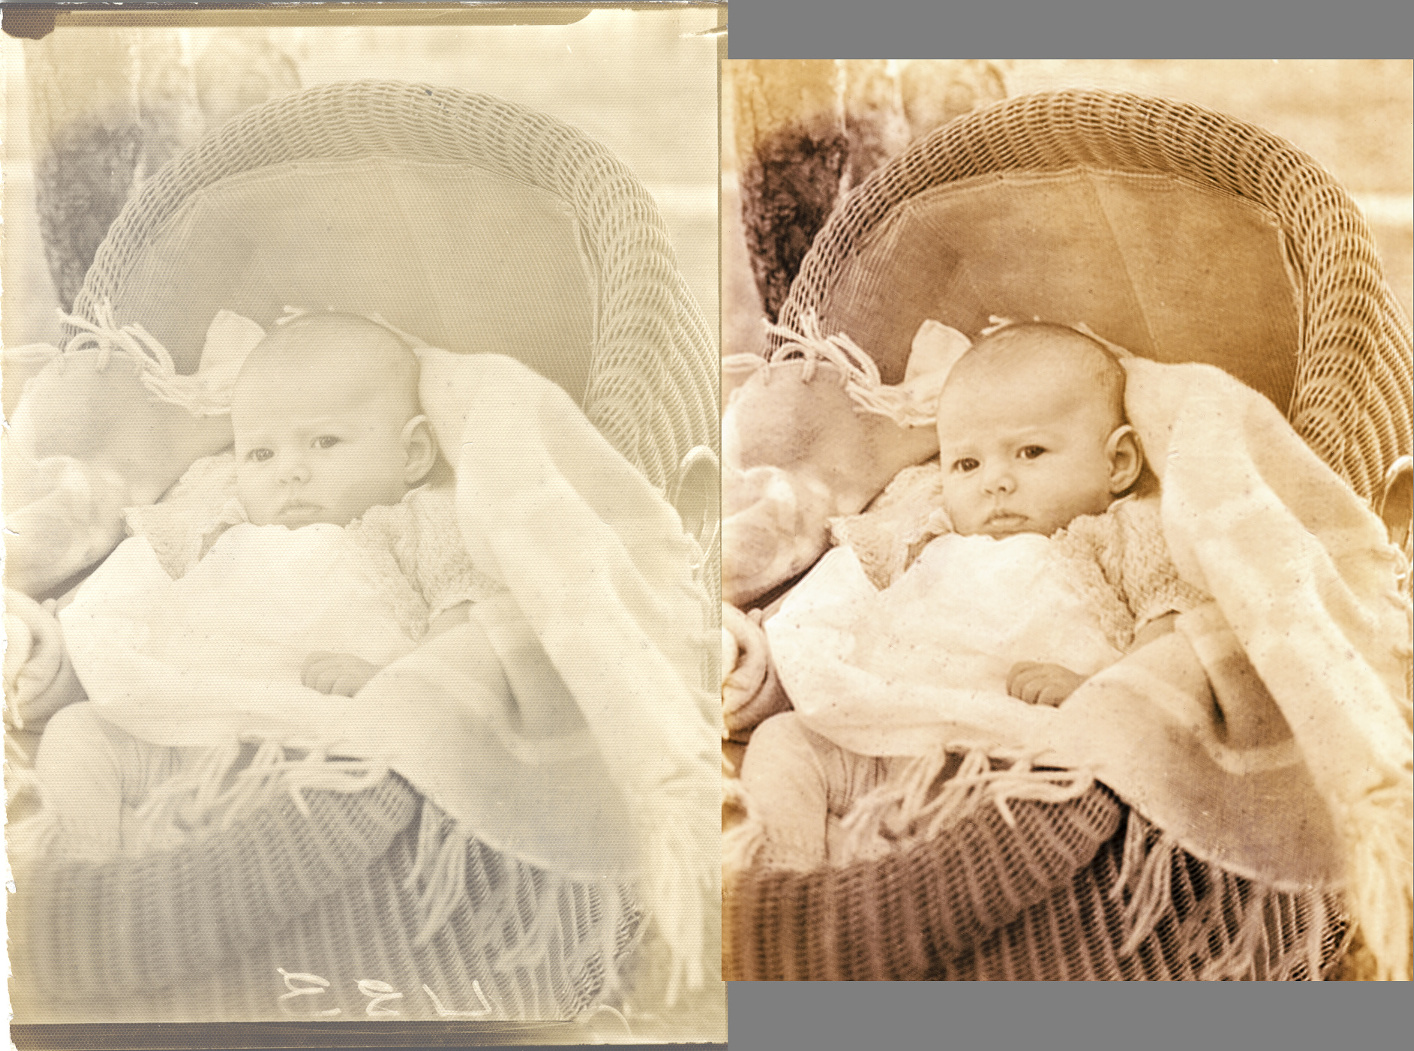
\includegraphics[width=6.08333in,height=4.52083in]{babyevelynbeforeafter.jpg}}
\caption{For some restorations, the ones that please or annoy me, I create a
before and after diptych. I want to convince myself that my restoration
work was worthwhile. Most of the time the restored image is better but
in more cases than I would like the original scan is superior. And, now
and then, I cannot decide which one I like the best. This rendering of
an old faded patterned print of my mother as a baby is one of those
images. The original print is on patterned paper. The pattern imparts a
quality that the restoration lacks. Ansel Adams once wrote that the
negative is the score and the print is the performance. For restorers,
the scan is the score and the restoration is the performance. Sometimes
the music is glorious and clear and sometimes it's rap -- rhymes with
crap!}
\label{fig:5317X3}
\end{figure}



%\section{Affinity Conclusion}

\medskip
\noindent\textbf{Affinity Conclusion}
\medskip

Affinity, like PWP, is a great value. The first Windows version is
already superior to every version of Photoshop Elements I've ever used.
It's not as comprehensive as full Photoshop, but if you subtract the
marginal features of Photoshop and keep the essential core elements,
you've basically described Affinity's feature set. Affinity is a layer
editor but it's not a Photoshop clone. The UI is completely modern, RAW
development is built in, sixteen-bit layers are the default, and useful
stack operations like automatic alignment are a click away. Affinity
also supports \href{https://vimeo.com/192633552}{thirty-two-bit HDR}
file formats and high dynamic range composites. There's a lot of bang
for the buck: strongly recommended!

%\begin{center}\rule{0.5\linewidth}{\linethickness}\end{center}

%\begin{enumerate}
%\item
%  \hypertarget{fn1}{}
%
%  If you remember what happened to Goliath siding with David doesn't
%  seem like much of a risk.\protect\hyperlink{fnref1}{↩}
%\end{enumerate}



%\end{document}